\documentclass[norsk,a4paper,12pt]{article}
\usepackage[T1]{fontenc} %for å bruke æøå
\usepackage[utf8]{inputenc}
\usepackage{graphicx} %for å inkludere grafikk
\usepackage{verbatim} %for å inkludere filer med tegn LaTeX ikke liker
\usepackage{mathpazo}
\usepackage{listings}
\bibliographystyle{plain}
\usepackage{xcolor}
\usepackage{float}
\usepackage{amsmath}
\usepackage{hyperref}

\setlength{\parindent}{0em}

\definecolor{background}{gray}{0.9}
\definecolor{comment}{rgb}{0.6,0.4,0.8}
\definecolor{string}{rgb}{0.6,0.4,0.8}
\definecolor{keyword}{rgb}{0.9,0.17,0.31}
\lstset{
	title=\lstname,
	numberstyle=\tiny, 
	breaklines=true,
	tabsize=4,
	language=Python,
	morekeywords={with,super,as},,
	frame=single,
	basicstyle=\footnotesize\tt,
	commentstyle=\color{comment},
	keywordstyle=\color{keyword},
	stringstyle=\color{string},
	backgroundcolor=\color{background},
	showstringspaces=false,
	numbers=none,
	numbersep=5pt,
	literate=
		{æ}{{\ae}}1
		{å}{{\aa}}1
		{ø}{{\o}}1
		{Æ}{{\AE}}1
		{Å}{{\AA}}1
		{Ø}{{\O}}1
	}


\title{Project Fys3600}
\author{Candidate numbers: 1. \& 14.}
\date{\today}
\begin{document}

\maketitle

\begin{figure}[H]
	\begin{center}
		
\includegraphics[scale=1.0]{Figures/uiosegl.png}
	\end{center}
\end{figure}



\newpage

\tableofcontents

\section{Introduction} % (Introduction to project and theoretical background)
\label{sec:intro}
	As society moves towards more automatization, accurate, globally available navigational tools are coming in demand. A solution to this is using satellites. 			There are some problems however. Satellites (and in some cases even earthbound equipment) are susceptible to bad space weather. Having your self-			driving car suddenly acting up is not desirable. Predicting when equipment will be in danger of getting hit by high energy particles is therefore of interest.\\ 
	\\
	In this report, we will be looking at data from several instruments measuring properties of the solar wind and the interplanetary magnetic field (IMF) along 			with auroras and some ionospheric currents.  We will also be looking at some potential consequences of the measurements.




\newpage
\subsection{Theory} % (The theoretical part of the intro)
\label{sub:theory}
	\subsubsection{The Sun:} 
		The root of all our problems is the star in the center of our solar system: the sun.\\
		\\
		\textbf{IMF}\\
		The sun, like the earth, has a magnetic field. This magnetic field stretches throughout the solar system, and has fittingly been dubbed the 						interplanetary magnetic field. What causes this magnetic field is beyond the scope of this report, but it is seemingly quite erratic, changing changing 				sign and field strength often.\\
		Something more constant about the imf is the general direction of the field lines. Due to the rotation of the sun, the magnetic field lines end up looking 			like archimedian spirals (or a ballerina skirt in 3 dimensions).
		\begin{figure}[H]
			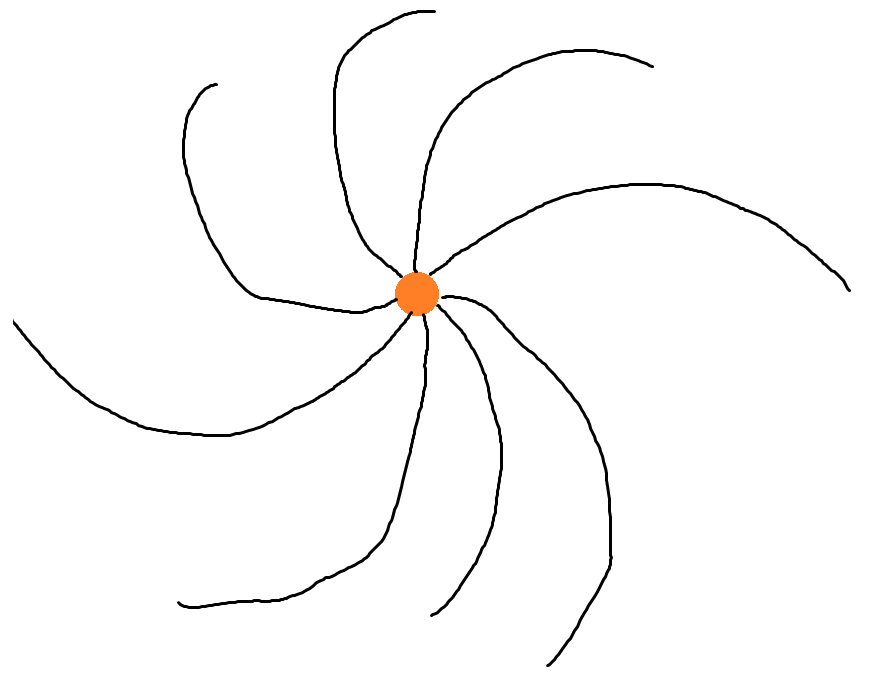
\includegraphics[scale = 0.3]{Figures/artistic_imf.png}
			\centering
			\caption{An artistic rendition of the interplanetary magnetic field. With the sun in the middle and rotating, the magnetic field lines end up forming 					     archimedian spirals.}
			\label{fig::spirals}
		\end{figure}

		\textbf{Solar Wind}\\
		Accompanying the magnetic field lines is plasma streams. Ejected from the suns corona, these plasma streams of varying velocity and density can also                         		be drawn like figure \ref{fig::spirals}.\\
		Carrying large amount of highly energized ionized particles, the solar wind is of great interest to us. Knowing the density and velocity of the solar wind 				is necesarry in understanding the consequences of its interactions with earth and its satellites.\\
		\\
		\textbf{Coronal mass ejection and solar flares}\\
		There are events where the sun sends out relatively huge amounts of plasma and radiation.\\
		One such event is a solar flare. A solar flare is a massive outburst of radiation happening in the lower corona. Being composed of mostly photons, a 				solar flare does not follow the magnetic field lines.\\
		Another such event is a coronal mass ejection (CME). During times of magnetic unrest, the sun might eject massive amounts of mass from its corona. 				Such outbursts are sometimes several times larger than the sun in diameter. The mass ejected follows the magnetic field lines, and ends up causing a 		spike in the solar wind density, something that can be harmful to instruments on earth.
		\begin{figure}[H]
			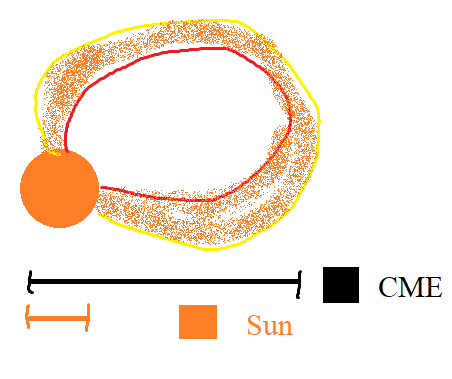
\includegraphics[scale = 0.7]{Figures/artistic_cme.png}
			\centering
			\caption{Artistic size comparison between the sun and a possible cme. As one can see, the cme can be many times larger in size than the sun.}
			\label{fig::cme}
		\end{figure}

\newpage
	\subsubsection{The Magnetosphere:}
		Like the sun, the earth also has a magnetic field.
		\begin{figure}[H]
			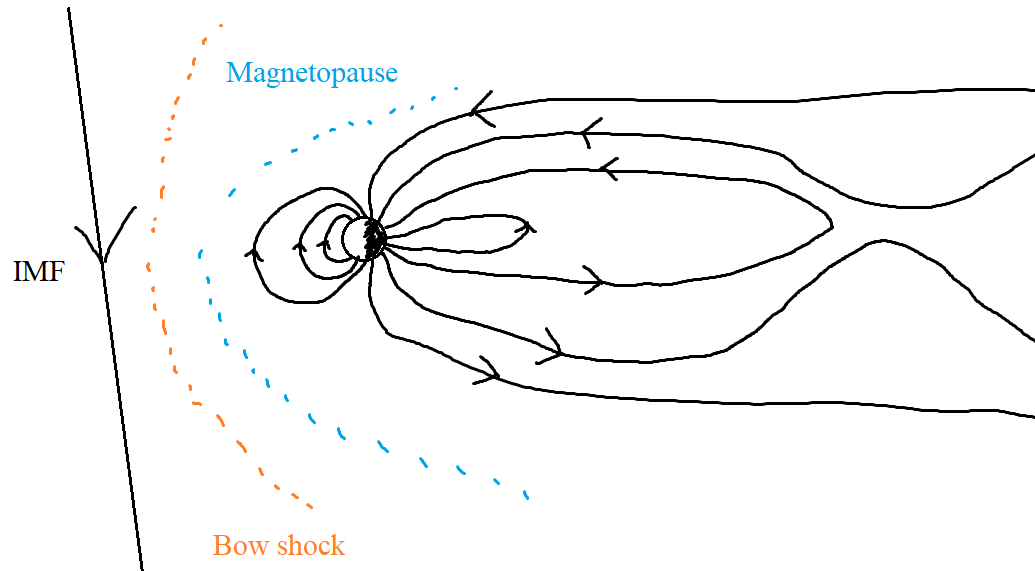
\includegraphics[scale = 0.5]{Figures/magnetosphere.png}
			\centering
			\caption{The earths magnetosphere. Note that it looks a bit different when the IMF Z component has the same sign as earths (in the figure, they 						     are opposite).}
			\label{fig::magnetopause}
		\end{figure}
	
	The earths magnetic south pole is currently located on the north pole. This means that the magnetic field goes from the geographical south pole to the 			geographical north pole. In figure \ref{fig::magnetopause}, this is indicated by arrows pointing along the field lines.  
% subsection theory (end)

% section introduction (end)


\section{instruments} % (description of the instrumenst used in this project)
\label{sec:instruments}




% section instruments (end)

\section{Observations} % (Detailed description of our observations, with all the graphs and figures nescessary)
\label{sec:observations}



 
% section observations (end)


\section{Discussion} % (Discussion of the results we got with respect to the observations)
\label{sec:discussion}

We got a bunch of shit here
% section discussion (end)

\section{Conclusion} % (Conclusion of the discussion and project)
\label{sec:conclusion}

Conclude some shit!
% section conclusion (end)



\section{Appendix} % (fold)
\label{sec:appendix}

% section appendix (end)

\section{Refrences and acknowledgements} % ()
\label{sec:refrences_and_acknowledgements}

% section refrences_and_acknowledgements (end)
\end{document}